\documentclass[main.tex]{subfiles}

\begin{document}
\section{Control System Design Methodology}
\textit{This section covers design methodology for control systems and software design. The focus is on the \gls{scada} architecture, how it is constructed and the methodology behind creating such a system. Finally, a discussion is made on the methodology of software design and common ways to structure code.}

The Readout units and the power supply board both require a software end point that essentially controls the entire system. This entails creating a system that can setup and configure the various parts of the system and also monitoring the system and report errors, i.e. we need to create a monitoring and configuration system.

\subsection{Overview}
Control systems have been a part of the industry for decades, it started in 1960s, where specialized minicomputers interfaced directly with devices in the plant or factory\cite{scada_history}. These systems were primarily used for automation, but they were highly specific and integrated to its system, using proprietary communication protocols and technology. Later, programmable controllers were starting to phase out minicomputers and \gls{hmi} have evolved from terminals with keyboards, to advanced \gls{gui}s. Ethernet eventually became the industry standard communication protocol. These technologies converged to a single system, such as system was nicknamed \gls{scada}.


A control system is generally is made out of sensors, a controller to control and retrieve data from the sensors, a supervisory computer that manages the process for the sensors, and \gls{hmi} software. The \gls{hmi} software provides access to the data from the sensors to the user and if needed, also allow the user to modify processes in the system.


\subsection{SCADA systems}
 \gls{scada} systems have five main functions: data collection, network data communication, data presentation, and remote monitoring and supervisory control\cite{scada_intro}. Although today, many control systems is based on \gls{iot}, which has a similar architecture. However, \gls{iot} bases itself on utilizing cloud-networking and processing for its communication infrastructure. Due to lack of wireless communication in the \gls{pct}-project, focus will be on how \gls{scada} systems are developed, although many of the same principles applies for both.

A \gls{scada} system typically is made out of five components:

\begin{itemize}
    \item Field devices and signals
    \item \acrfull{ppc}
    \item \acrfull{hmi}
    \item Database servers
    \item Communication infrastructure
\end{itemize}

Field devices and signals encompasses all sensors and the actuators that controls them. \gls{ppc} is responsible for automatically controlling the field devices, as well as retrieving data from them and send it to the \gls{hmi}. A microcontroller is an example of a \gls{ppc}. \gls{hmi} is the software being executed on the main computer and is made of a user interface and database manager. The \gls{hmi} serves as the interface for the user to set up configuration processes and monitor the system performance. For this purpose, a configuration database is required to set up the \gls{ppc}s with correct values, and a historical database is needed to store monitoring data from the field devices. A communication infrastructure connects the \gls{ppc}s to the workstations running the  \gls{hmi} software. An image of a typical \gls{scada}-system is shown in \autoref{fig: scada_system}.

\begin{figure}[!ht]
    \centering
    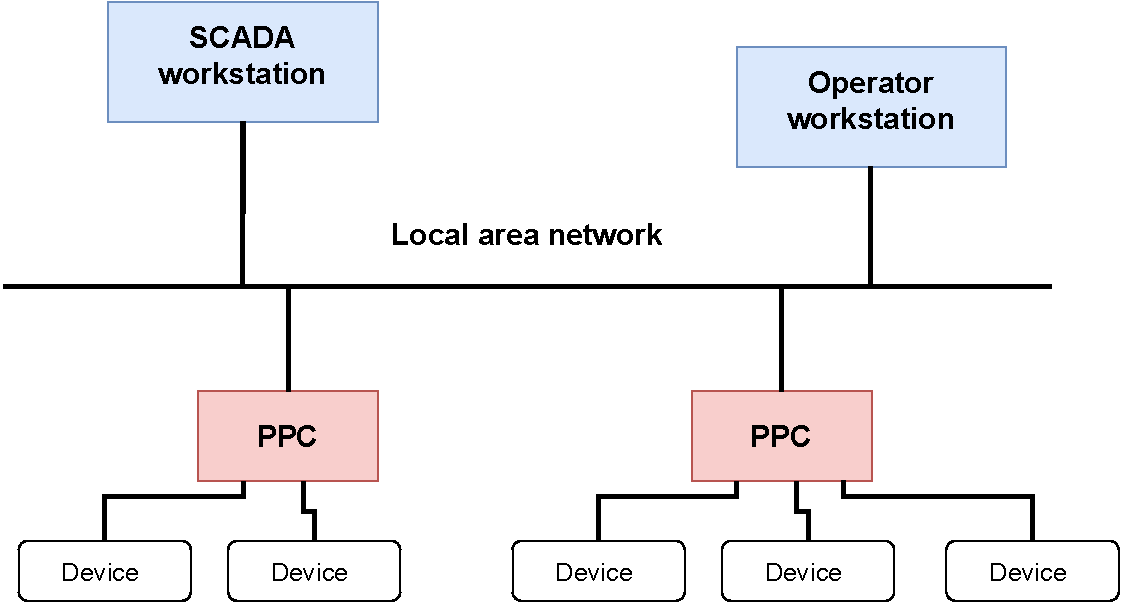
\includegraphics[scale=0.6]{images/scada_system.pdf}
    \caption{Block diagram of a typical SCADA system, based on diagram from\cite{scada_design}.}
    \label{fig: scada_system}
\end{figure}
\FloatBarrier

The image shows field devices, connected to \gls{ppc}s that controls them. The \gls{ppc}s are connected to the \gls{scada} \gls{hmi}, or smaller operator \gls{hmi}s through a local area network. The \gls{ppc}s are usually connected to a Local area network, where they send and retrieve data to the  \gls{hmi}s. The \gls{hmi} interfaces with the database server to process configuration and monitoring data, although some systems allow the \gls{ppc} to directly access the database.


\subsection{SCADA software development}

The life cycle of a \gls{scada}-system project is important to understand in order to create a similar system. The methods involved in creating a typical \gls{scada}-system ensures the software and its documentation becomes well organized and structured.

\subsubsection{Project specifications}

Before starting to design a \gls{scada}-system, the requirements of the project must be understood. This includes, but are not limited to\cite{scada_design}:

\begin{itemize}
    \item Diagram of system architecture
    \item Specifications for field controllers and Human to Machine interface
    \item Identification of input and output signals for each controller

\end{itemize}

 Diagrams of the process and the instruments in the the system gives an overview and understanding of the project specifications. One must understand what function the \gls{ppc} and the \gls{hmi} will have in the system.  the input and output signals of the controllers must be specified, which is the measurements retrieved from the controllers, and the configuration values of the controllers.

\subsubsection{Input and output signals}

A list must be made of the input and output signals of a system. Knowing all signals to be used in a system will give us an estimate of the requirements of the system as well as aid in the development process. 
The input and output signals determines the configuration and monitoring processes. The input signals affect how the \gls{ppc} will control the field devices. These can be discrete values which determines if a valve is open or closed, or it can be analog signals which determines voltage thresholds in a circuit. The output signals are the values to be monitored by the \gls{ppc} which are polled by the \gls{hmi}, and stored in a database. These are usually measurements from a sensor, such as temperature, voltage, or flow.

\subsubsection{Developing Workstation software}

The software to be used in the Workstations is comprised of two parts, the graphical display of the system, which serves as the \gls{hmi}, and the databases containing information of the \gls{ppc}s. The Graphical display must be designed in such a manner that the user can quickly and easily survey and control the system. Security must also be considered in the design, certain functions that can change parameter values should ideally be only for available to administrative users. This is to reduce the chance of equipment or instruments being damaged by inexperienced users.

The database software must store configuration values for the \gls{ppc}s, as well as storing the monitoring data from them. There is usually two databases maintained for this purpose, one for configuration, and one for monitoring. Communication software must be developed that regularly polls data from the \gls{ppc} and inserts it into the monitoring database. Likewise, the configuration software must retrieve data from the configuration database and send the data to the \gls{ppc}.



\subsubsection{Software documentation}
Another important aspect of such a control system is having a consistent programming standard and complete software documentation. \gls{scada} and similar systems often have a long shelf time, and a well documented system will make maintenance and work in the future be much easier. In general, starting with good software documentation and expanding upon it during the project development will lead to sufficient documentation of the entire system.

A consistent programming standard helps in debugging and in expanding functionality of the system. \gls{oop} is a very common programming paradigm that is used to give structure to programs and increase reusability and maintainability of the code. Systems designed to manage large data acquisition, such as a \gls{pet}-scan system, have in the past used \gls{oop} to design and manage large programs\cite{pet_control_system}, this suggest that this programming structure is viable for the design of the control system in the \gls{pct}-project.


\subsection{Software design}

\subsubsection{Git and GitHub}

The use of the Git and GitHub tools is essential today to manage your code, maintain it and also as a version control system. Git is another method used to ensure that the code is easy to use and be maintained, now and in the future. The version control system is also essential for verifying the code, mistakes can be made, but a stable version of the software will always be available at the GitHub. GitHub also enables a better workflow with co-developers or mentors, allowing easy access to the source code and issues can be made. There is currently only one master branch of the repository in the Git system, this is due there only being one developer so branching is not yet needed.

The GitHub repository contains a README-file which contains all practical information about the repository and the goals of the project. This includes information about the configuration and monitoring process, as well as a user guide to start the databases and \gls{gui}. An example of the README-file is given in \autoref{fig: readme}


\begin{figure}[!ht]
    \centering
    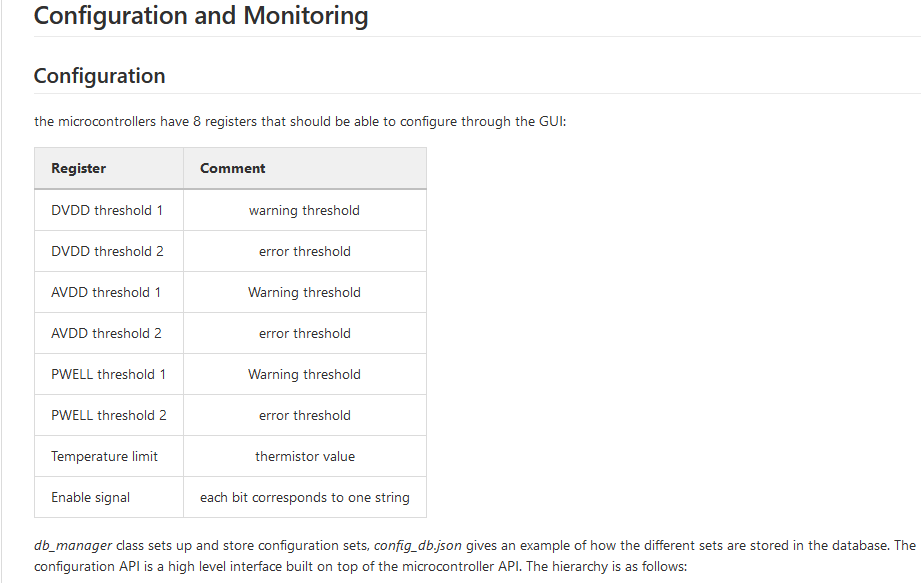
\includegraphics[width=18cm]{images/README_example.png}
    \caption{Example from the README-file showing the overview of the configuration process.}
    \label{fig: readme}
\end{figure}
\FloatBarrier

\end{document}

\end{document}